\documentclass{article}
\usepackage[a4paper, margin=1.5in]{geometry}
\usepackage[utf8]{inputenc}
\usepackage[T1]{fontenc}
\usepackage{hyperref}
\usepackage{palatino}
\usepackage{adjustbox}
\usepackage{graphicx}
\usepackage{booktabs}
\usepackage{minted}
\setminted{fontsize=\footnotesize}
\setcounter{tocdepth}{2}

\title{Extending MLKit with vector instructions}
\author{Christian Kjær Larsen}


\begin{document}

\maketitle

\tableofcontents

\section{Introduction}

In this section we will briefly describe the project, its purpose and the structure of this report.

\subsection{Project statement}

The goal of this project is to add packed vector support to the MLKit\cite{mlkit} Standard ML compiler using the AVX2 vector instructions present in modern Intel processors. The motivation is to be able to use this support to optimize programs written in Standard ML to exploit data parallelism.

\subsection{Road-map}

\begin{enumerate}
    \item We start by investigating other approaches to SIMD (Single Instruction Multiple Data) programming in higher level languages. This is in order to settle on a
        good abstraction that is fairly easy to program with.
    \item
        We then continue by designing a programming abstraction to be able to optimize a program in a generic way that is not tied to a particular instruction set or set of vector extensions.
        We also write some simple example programs that will work as motivating examples and show that the abstraction is actually useful.
    \item
        Finally we implement compiler support for Intel AVX in the MLKit Standard ML compiler by providing a set of intrinsics that compile to efficient code that use native vector instructions.
\end{enumerate}

\subsection{Source code}
We have included two archives with source code. One is the source code of the forked MLKit compiler, and the other is the libraries, example programs and benchmarks written while completing this project. An overview of the source code and the changes can be found in the appendix.

\section{Background}

In this section we will motivate the project by giving some background on vector extensions in modern CPUs and how one would typically accelerate a program using vector instructions is mainstream programming languages.

\subsection{Vector instructions in modern CPUs}

Ordinary instructions in a modern CPU typically work on one or more registers each containing scalar values. For instance, the following X86-64 program will increment a number, and store it to memory:
\begin{minted}{gas}
addq 0x1, %rax
movq %rax, (%r10)
\end{minted}
During the 90s, the demand for doing signal and image processing on desktop computers increased, and CPUs designers began adding vector instructions to their processors. Image processing typically requires the same operations to be performed, say, for each pixel in an image. An efficient way to do this, is to add instructions that perform the same instruction on wider registers containing for instance 4 single-precision floating point numbers.

On modern Intel CPUs we typically have access to an number of vector extensions. Popular ones include:

\textbf{SSE2 (Streaming SIMD Extensions 2)} gives us 128 bit registers that can contain 8 to 64 bit integers, single and double-precision floating point.

\textbf{AVX2 (Advanced Vector eXtensions 2)}
that gives us 256 bit registers, and adds instructions that operate on 3 registers not overwriting one of the arguments. This allows for more compact code. The following program will multiply two vectors of four 64-bit integers and store them to memory in two instructions using AVX instructions:
\begin{minted}{gas}
vpaddq %ymm0, %ymm1, %ymm2
vmovdqa64 %ymm2, (%r10)
\end{minted}

On ARM there are also vector extensions:

\textbf{Neon}
allows up to 128 bit vectors of both integers and floating point.

\textbf{SVE (Scalable Vector Extension)}
is a variable length vector extension designed for high-performance computing, and it allows vector lengths from 128 to 2048 bits.

Other modern instruction sets like PowerPC, RISC-V and SPARC also include their own vector extensions.

\subsection{Programming model and higher level languages}
Programmers do not usually write the assembly code directly, but rely on different high level constructs.

\subsubsection{Intrinsics}

The primary way that people program with vector instructions is by using intrinsics. Compilers include C-libraries with intrinsic functions that are guaranteed to compile to vector instructions under the hood. For instance in the Intel C compiler, we can use the function
\begin{minted}{c}
#include <immintrin.h>
__m256d _mm256_add_pd (__m256d a, __m256d b)
\end{minted}
to add together two vectors of 4 double-precision floating point numbers. In the library, the type \verb!__m256d! represents a packed vector register of 4 doubles. These abstractions make it fairly easy to program with vectors, but a problem is that the implementations are highly tied to the particular instruction set. To target for instance ARM, you would have to rewrite the program entirely.

\subsubsection{LLVM}

LLVM\footnote{\url{https://llvm.org/}} is a popular intermediate language used in a lot of modern compilers. It natively supports vector instructions, and has multiple back-ends that target different instruction sets. This means that if a high level language targets the LLVM, then making a portable vector library is fairly easy.

For instance Rust targets the LLVM intermediate language which. It provides a standard interface\footnote{\url{https://github.com/rust-lang/stdsimd}} to generic functions on vectors that are lowered directly to LLVM and compiled for specific architectures there. This means that you can write a function that works for vectors of, say, 4 64-bit floats, and then it would be lowered to the LLVM type \verb!<4 x double>!. The problem of choosing good instruction for certain operations are then delegated to the LLVM back-end.

\subsubsection{.NET and Java}

Lately also higher level languages like C\# and Java have added support for vector instructions.

Recently, Microsoft added the library \verb!System.Numerics.Vector!\footnote{\url{https://docs.microsoft.com/en-us/dotnet/api/system.numerics.vector}} such that C\# programmers could accelerate their programs the SIMD instructions of modern CPUs.

The library makes it possible to write programs that are generic in both vector types and vector lengths. Then the JIT-compiler will use vector instructions if they are supported on the host, otherwise there will be a fallback to a slower implementation using regular instructions.

A similar thing will be added to the JVM in version 16\footnote{\url{https://openjdk.java.net/jeps/338}}.

Both the .NET and the JVM implementations will have to be platform agnostic, since both of them compile to intermediate code that has no knowledge of the architecture on which it runs. This means that the run-time will JIT-compile intermediate code to vector instructions only if they are supported on the host.

\subsubsection{Challenges}

One major challenge is not to tie the implementations to tightly to the specific instruction set. It should be fairly easy to change a program from say AVX2 to Neon. This then gives the problem of instruction selection. Do you expose direct versions of the AVX2 instructions, and then make other instruction sets emulate those, or do you try to find a common ground, that makes useful operations with good performance available on all CPUs. This is some of the problems faced by the designers of the JVM and .NET vector APIs, and we will try to consider some of the same issues.

Take for instance the sum of a vector with 4 elements,
\[
    \mathtt{sum}\ [a_1, \ldots, a_4] = a_1 + \cdots + a_4.
\]
The AVX2 instruction set has no direct support for such an operation, and the most efficient implementation might depend on vector sizes and element types. The proposed RISC-V vector extensions directly expose a \texttt{vfredsum.vs} that directly reduces a vector. If we looked at the Intel instruction set, we would probably not include this operation, since there is no simple efficient way to implement it. If we would focus on the proposed RISC-V vector extensions, we would add it without hesitation.

Since we in this project only focus on MLKit's 64-bit Intel back-end, we restrict ourselves to vectors of 4 reals (64-bit floats). This is supported by AVX2 which is widely supported now. We will of course keep in mind to design our library such that it is not too tied to AVX2.

\section{Design of a vector signature}

In this section we will briefly describe a vector signature that can be used for SIMD programming in SML. We will also show how to write simple programs that use it.

\subsection{Generic interface}

We have created a \verb!REAL4! signature that will operate on a packed vector of 4 \verb!real!s. An overview can be seen on listing~\ref{lst:real4}.
\begin{listing}[ht]
\begin{minted}[frame=single]{sml}
signature REAL4 = sig

  type element = real
  type interface = real * real * real * real

  type simd
  type mask

  val mk : interface -> simd
  val read : simd -> interface

  val broadcast : element -> simd

  (* arithmetic operations (vectors and scalars) *)
  val add : simd * simd -> simd
  val adds : simd * element -> simd
  (* and so on *)

  (* comparisons (vectors and scalars) *)
  val lt : simd * simd -> mask
  val lts : simd * element -> mask
  (* and so on *)

  (* operations on masks *)
  val and_ : mask * mask -> mask
  val or_ : mask * mask -> mask
  val not_ : mask -> mask

  (* reductions *)
  val all : mask -> boolean
  val any : mask -> boolean
  val sum : simd -> element
  val product : simd -> element

  (* conditional operations *)
  val blend : simd * simd * mask -> simd
end
\end{minted}
\caption{\texttt{REAL4} vector signature}
\label{lst:real4}
\end{listing}

There are two opaque types. \verb!simd! represents the actual vector and \verb!mask! represents a vector of booleans that can be the result of comparisons. We have chosen to fix the number of elements in the signature, since this makes the signature much easier to use. An alternative would be to make the \verb!mk! and \verb!read! functions work on lists, and then we could reuse the signature to work on multiple vector lengths. This of course makes the interface more fragile.

We include arithmetic operations both in vector-vector and vector-scalar form. The comparisons will return masks where the individual elements correspond to the comparison between individual elements. We also include common boolean operations on masks.

To collapse vectors into elements, we also include some reductions. \verb!sum! and \verb!product! will collapse an entire vector into the sum or product of its elements. \verb!all! and \verb!any! will return true if all or any of its elements are true. Other reductions could also be added in the future like minimum and maximum.

A signature for packed integers \texttt{INT4} could also be added, and an implementation could also be made using AVX2 instructions, but we have chosen to focus on floating point in this project.

\subsection{Pure SML structure}

It is pretty easy to implement a pure SML structure that we can use to test our hardware accelerated version against. We just use tuples of reals for vectors and tuples of booleans for masks. A part of such an implementation can be seen on listing~\ref{lst:tup}.
\begin{listing}[ht]
\begin{minted}[frame=single]{sml}
structure Tup4 : REAL4 = struct
  type simd = real * real * real * real
  type mask = bool * bool * bool * bool

  fun mk a = a
  fun read a = a

  fun broadcast v = (v, v, v, v)
  fun all (m1, m2, m3, m4) = m1 andalso m2 andalso m3 andalso m4

  (* And so on *)
end
\end{minted}
\caption{Implementation of \texttt{REAL4} using tuples}
\label{lst:tup}
\end{listing}
The entire implementation is included in the source code.

\subsection{Writing programs}

Writing a simple numeric program using this structure is very easy, since the \verb!simd! values are almost interchangeable with reals.
\begin{minted}{sml}
fun foo (x: real, y: real) = x*x + y*y

fun foo_simd (x: simd, y: simd) = add (mul (x, x), mul (y, y))
\end{minted}
We can write programs with conditionals by using the \texttt{blend} operation. It gives us the possibility to select from one of two vectors based on a mask. We can use it to write a vectorized version of a maximum function:
\begin{minted}{sml}
fun max (v1: real, v2: real) = if v1 < v2 then v2 else v1

fun max_simd (v1: simd, v2: simd): simd =
  blend (v1, v2, lt (v1, v2))
\end{minted}
\texttt{blend} will select elements from the first vector when the element in the mask is true, and otherwise take the element from the second vector.

If we want to write a loop that terminates based on some condition about elements of the vector, we can use the boolean reductions to make a predicate about the entire vector.
We can for instance make a tail recursive function that adds 1.0 to each element until all elements are above 9000.
\begin{minted}{sml}
fun loop (x: simd): simd =
  if all (gts (x, 9000.0))
    then x
    else loop (adds (x, 1.0))
\end{minted}

\subsubsection{Vectorizing Mandelbrot}

Using these building blocks, we can try to rewrite a larger program to use the vectorized operations. We will take a look at a simple implementation of a function that calculates whether a complex number belongs to the Mandelbrot set\footnote{OK. Formally we calculate how many iterations it takes to converge, and then we assume it diverges is it requires more than 1000 iterations. We typically only use this algorithm to color pixels in a nice image.}.
\begin{minted}{sml}
fun mandelbrot (re: real, im: real): int =
  let
    fun go iter x y =
      if (re*re + im*im <= 4.0 andalso iter < 1000)
      then go (iter + 1) (re*re - im*im + x0) (2.0*re*im + y0)
      else iter
  in
    go 0 0.0 0.0
  end
\end{minted}
A way to approach vectorizing it is to consider 4 values at a time $(x_1, y), \ldots, (x_4, y)$. The problem is that for 4 pixels it might be the case that some diverge and some converge. We can use masks to essentially block the updates for pixels that have converged already.

\begin{minted}{sml}
functor Mandelbrot(Real4 : REAL4) = struct
open Real4
fun mandelbrot_simd (re: simd, im: real): simd =
  let
    val zero = broadcast 0.0
    fun square x = mul (x, x)
    fun go (iter, iters, re', im') =
      let
        val re2 = square re'
        val im2 = square im'
        val mask = les (add (re2, im2), 4.0)
      in
        if (any mask andalso iter < 1000)
        then
          let 
            val re'' = add (sub (re2, im2), re)
            val im'' = adds (muls (mul (re', im'), 2.0), im)
          in
            go ( iter + 1
               , blend (iters, adds (iters, 1.0), mask)
               , blend (re', re'', mask)
               , blend (im', im'', mask)
               )
          end
      else iters
    end
  in
    go (0, zero, zero, zero)
  end
end
\end{minted}
We start by computing the mask that corresponds to the condition in the original if-statement. If all values are false, we stop iterating, since all values in the vector has either converged or diverged. We then use the \verb!blend! operation to conditionally update only the iteration count and the temporary values for those elements where the if-condition in the original program would have been true.

Rewriting a program like this is a bit mechanical, and could maybe be done automatically for these kinds of functions with some meta-programming or complicated array library.

Running this code now with our mock implementation of vectors using tuples is a bit silly, so we will now implement AVX2 support in the MLKit to hopefully get this code running fast.

\section{Implementation in the MLKit}
In this section we will describe the changes made to the MLKit compiler in order to support the vector operations described in the previous section using AVX2 instructions. The internals of the MLKit is not super documented, so there will be a lot of mentions of concepts in the compiler that has no references, and is simply understood by reading through the code base.

\subsection{Types}
We will represent vectors and vector masks in MLKit as strings. This means that the default representation of vectors will be boxed, and we can therefore easily use vectors in generic functions and have them garbage collected and so forth. This will make operations on vectors fairly inefficient though, since will will have to load and store them every time we do a vector operation. We will solve some of these inefficiencies later in this section. 

\subsection{Primops}
The way that the programmer will have access to native vector instructions is through the \texttt{prim} feature of MLKit. In a library we can call a primop, and then we can generate native code in the code generator for that particular primop, and get efficient machine code for particular operations.

On table~\ref{tbl:primops} an overview of the added user facing primops can be seen.
\begin{table}
\begin{adjustbox}{width=\columnwidth,center}
\begin{tabular}{l l l}
    \toprule
    Category & Primop & Type \\
    \midrule
    Arithmetic & \verb!__m256d_plus! & \verb!string * string -> string! \\
                & \verb!__m256d_minus! & \verb!string * string -> string! \\
                & etc. & \\
                \midrule 
    Logic       & \verb!__m256d_and! & \verb!string * string -> string! \\
                & \verb!__m256d_not! & \verb!string -> string! \\
                & etc. & \\
                \midrule 
    Conditional & \verb!__m256d_le! & \verb!string * string -> string! \\
                & \verb!__m256d_blend! & \verb!string * string * string -> string! \\
                & etc. & \\
                \midrule 
    Reductions  & \verb!__m256d_all! & \verb!string -> bool! \\
                & \verb!__m256d_sum! & \verb!string -> real! \\
                & etc. & \\
                \midrule 
    Load and store & \verb!__m256d_broadcast! & \verb!real -> string! \\
                   & \verb!__m256d_true! & \verb!unit -> string! \\
                   & \verb!__blockf64_update_m256d! & \verb!string * int * string -> unit! \\
                   & \verb!__blockf64_sub_m256d! & \verb!string * int -> string! \\
                   & etc. & \\
                   \bottomrule
\end{tabular}
\end{adjustbox}
\caption{Overview of added primops}
\label{tbl:primops}
\end{table}

We steal the naming convention from Intel that \texttt{m256d} is a 256 bit vector of double-precision floating point numbers. The user facing type of vectors is \verb!string! which is chosen, since in the compiler it is a type that roughly corresponds to an array of bytes. We can hide this type in a structure which implements the \texttt{REAL4} signature by using opaque signature matching, so that the user does not accidentally concatenate it with a string.

Most of these operations correspond directly to the functions in the \texttt{REAL4} signature. Additionally we have added primops for dealing with unboxed arrays of reals. The \verb!__blockf64_update_m256d! primop will update 4 values at the specified index in a block of memory containing unboxed reals. The \verb!__blockf64_sub_m256d! will get the 4-element vector from the specified index. We have not added read and write masks to deal with conditional loads and stores, and we leave this as future work.
    
\subsection{Internal representation}

The MLKit has a boxed floating point representation accessible to the programmer as the \verb!real! type in Standard ML. Internally in the optimizer, unnecessary boxing operations are avoided by using unboxed operations directly on floating point registers thereby avoiding expensive memory operations in basic blocks. Due to the uniform memory representation, these unboxed floats can not be passed to generic functions and should therefore not be exposed to the programmer.

We will do something similar for our vectors. For the programmer all the vector operations work on strings since we did not extend Standard ML with new types. We add a new internal type, \texttt{F256} to the compiler. This is not visible to the programmer, and is only used when optimizing programs in the same way as the \texttt{F64} type is used for reals. Values of the type \texttt{F256} are stored in \texttt{ymm} registers just like \texttt{F64} values are stored in \texttt{xmm} registers.

\texttt{ymm} registers completely overlap with \texttt{xmm} registers, which means that we cannot just allocate vector registers independently from regular floating point registers. We have chosen to deal with this in a rather simple way. When using a vector instruction, we just request a regular floating point register from the register allocator, and have the compiler change the register to a \texttt{ymm} register when the instruction is written. This also gives us the flexibility to look at a 4 element vector register as having only one or two elements.

\subsection{Implementing boxed operations}

To implement the primops in table~\ref{tbl:primops} we take a pretty simple approach. We make unboxed versions of the primops that work on vector and floating point registers using the \texttt{F64} and \texttt{F256} types. We then insert explicit boxing operations around the result, and explicit unboxing operations around the arguments. In other words we can implement a boxed version of a function by rewriting it using a unboxed version
\[
    f_{\mathrm{boxed}} \equiv \mathtt{box}\ (f_{\mathrm{unboxed}} (\mathtt{unbox}\ x)).
\]
Then we only have to implement support for unboxed operations, and the complexity of dealing with memory allocation, loading and storing vector values to memory will be handled in the implementation of the the primops \verb!__f256_box! and \verb!__f256_unbox!. There are already primops for boxing and unboxing reals that we can reuse.

For instance we will implement \verb!__m256d_broadcast x! by rewriting it to
\begin{verbatim}
__f256_box (__f256_broadcast (__f64_unbox x))
\end{verbatim}
Also we will not generate code for the boxing operation for vectors. What we will do instead is to rewrite the boxing operation to the following code in the last step of the optimizer:
\begin{minted}{sml}
let
  val box = SCRATCHMEM 32
  val ()  = __f256_store (value, box)
in box
\end{minted}
Where \verb!SCRATCHMEM 32! is a primop that will allocate 32 bytes of uninitialized memory. Then the \verb!__f256_store! primop will do a single \verb!vmovupd! to store the content of the vector register in memory.

The reason why we have boxing as a distinct primops is, that we rely on elimination of boxing operations in the compiler to get decent performance. Manipulating intermediate code with explicit boxing operations is much simpler than manipulating stores and allocs as well.

\subsection{Instruction selection}

We now have one job to do before we can actually compile some code. We will select instruction sequences to generate for the unboxed primops.

\paragraph{Arithmetic and logic}
All the arithmetic primops and \verb!f256_or! and \verb!f256_and! can be implemented by a single instruction, and are very simple and efficient. Implementing \verb!not_f256! requires an \verb!xor! with a mask with all 1s. We can generate a mask with all 1s with the \verb!vpcmpeqd! instruction. It compares vectors for equality, and we can just compare any vector with itself.

\paragraph{Reductions}
The vector reductions are a bit more interesting. There is not great support in AVX2 for vector reductions, since the entire point of vector instructions is to operate on independent data.

We will implement support for \verb!__f256_any! and \verb!__f256_all! by using the \verb!vmovmskpd! instruction. It will move a mask register with the value
\[
    b_0 \ldots b_{255}
\]
into a general purpose register with by extracting the last bit of each of each element
\[
    b_{63}b_{127}b_{191}b_{255}0\ldots0.
\]
We can then implement \verb!any! by checking whether this bit string is different from 0 and we can implement \verb!all! by checking whether this bit string is equal to $1111$.

The reductions \verb!__f256_sum! and \verb!__f256_product! requires a few more instructions.

For the sum of a vector register \verb!ymm0! there is a few different ways to implement the reduction. We either have to use a horizontal add which will add together the top two elements and the bottom two elements. We then have to shuffle the elements around and do a scalar addition at the end. AVX2 has no horizontal multiplication though, so we have chosen another approach just so that the implementations for addition and multiplication are similar. The following instruction sequence will do a reduction with plus, and a reduction with multiplication can be achieved by replacing \verb!add! with \verb!mul!.
\begin{minted}{gas}
vextractf128 0x1, %ymm0, %xmm1 # (1)
vaddpd %xmm0, %xmm1, %xmm0     # (2)
vunpckhpd %xmm0, %xmm0, %xmm1  # (3)
vaddsd %xmm1, %xmm0, %xmm1     # (4)
\end{minted}
We have tried to visualize the shuffling around of elements on figure~\ref{fig:hadd}. The first instruction will extract the top two elements. The second instruction will add the bottom and the top together. The third instruction will extract the top element and the last instruction will do the sum in the bottom element. Here we also see an advantage of the overlapping vectors. We can use the same registers for scalars, two element vectors and four element vectors.
\begin{figure}
    \centering
    \caption{Implementation of sum}
    \label{fig:hadd}
    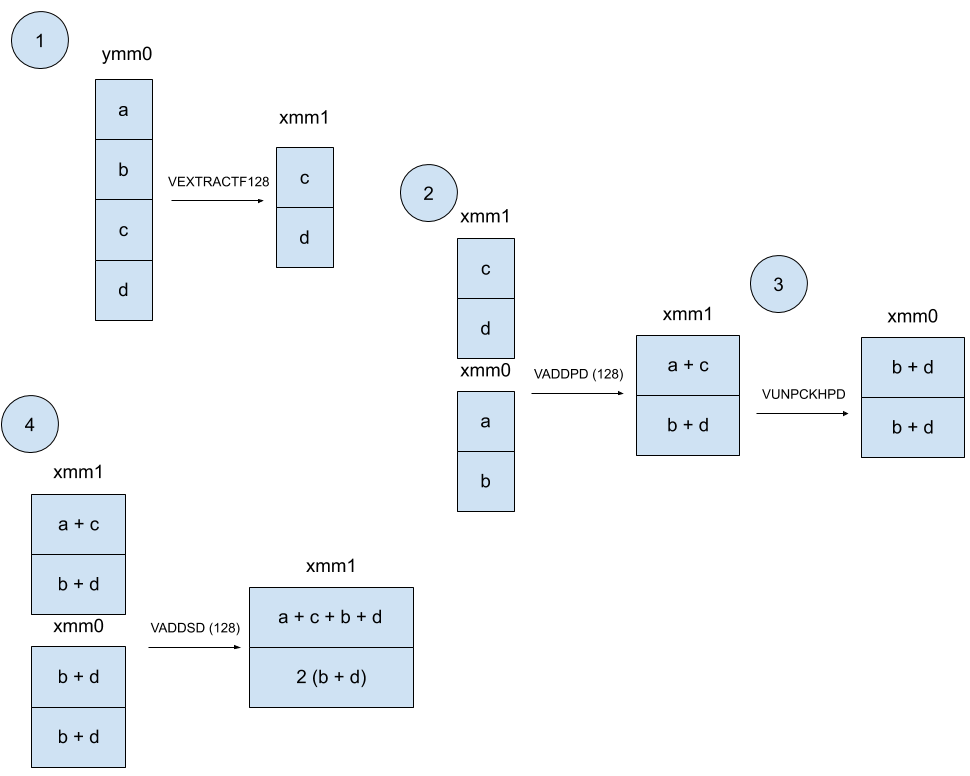
\includegraphics[width=0.7\textwidth]{sum.png}
\end{figure}

\paragraph{Comparisons and conditionals}
The usual comparison operations on x86 will set flags, and will not place a result in a register. For AVX, a comparison of two vectors will place the resulting mask in a vector register. This means that in order to implement the comparison primops, we only have to return the mask register, which makes them very simple to implement. They are all just a single instruction. We then have to use boolean reductions in order to put them inside an if-expression in SML.

Implementing \verb!__f256_blend! is just a single instruction. It takes to vectors and a mask, and writes to a result using the mask.

\paragraph{Loads and stores}

Implementing \verb!__f256_broadcast! is also only a single instruction. We can use the unboxing of reals already present in the MLKit for the argument.

We generate \verb!true! and \verb!false! constants using \verb!xor! or \verb!vpcmpeqd! with the same register to generate masks of 0s and 1s.

All memory accesses are just using a single \verb!vmovupd! instruction.

Since we did not want to modify the memory allocation in MLKit too much, we have made the decision to rely on the unaligned memory operations that are possible in AVX2. They might be a little slower than making sure that all accesses are properly aligned though.

Now we are actually able to generate functioning code, but the generated code will contain a very large number of boxing operations. We will try to optimize for those now.

\subsection{Unboxing}

Since our representation of vectors is boxed, then we will have quite a large overhead doing any operations on them. Every time we want to operate on a vector we have to unbox it, do the operation and box the result. That is quite costly. In order to generate efficient machine code, we want to get rid of unnecessary boxing operations. We will do two fairly simple optimizations for now.

\paragraph{Elimination of box-unbox and unbox-box}
If we do a series of vector operations in a row, we will have box and unbox operations in between. These can be easily eliminated by considering the equivalences
\[
    \mathtt{box} (\mathtt{unbox}\ x) \equiv x
\]
and
\[
    \mathtt{unbox} (\mathtt{box}\ x) \equiv x
\]
that we assume to hold for our boxing operations. The explicit unboxing and boxing of, say, compiling $(x + y) * (a + b)$ might give us the program 
\begin{minted}{sml}
box ( mul ( unbox (box (add (unbox x, unbox y)))
          , unbox (box (add (unbox a, unbox b)))
          ))
\end{minted}
We can then safely rewrite this to
\begin{minted}{sml}
box ( mul ( add (unbox x, unbox y)
          , add (unbox a, unbox b)
          ))
\end{minted}
Eliminating 4 boxing and unboxing operations.

\paragraph{Unbox let-binding of vectors}
The explicit boxing and unboxing might leave us with a program like
\begin{minted}{sml}
let
  val a = box (add (unbox x, unbox y))
  val b = box (mul (unbox x, unbox y))
in box (sub (unbox a, div (unbox b, unbox a)))
end
\end{minted}
This has a lot of unnecessary boxing operations that the previous optimization did not get rid of. If we know that a boxed let-binding is always used in an unbox operation in its scope, then we can safely eliminate those operations. We can rewrite the previous program to
\begin{minted}{sml}
let
  val a = add (unbox x, unbox y)
  val b = mul (unbox x, unbox y)
in box (sub (a, div (b, a)))
end
\end{minted}
which eliminates 5 boxing and unboxing operations and will give us fairly efficient straight-line machine code. These two optimizations are implemented in the optimizer for MLKit's intermediate language.

We can now go ahead and implement the \verb!REAL4! signature, and start to write Standard ML code that is optimized with AVX2 instructions.

\subsection{Signature using primops}

Since our boxed representation is the same as for unboxed arrays of reals, we can use the \verb!__blockf64! primop for making vector from tuples. Similarly we can index into the vector using the \verb!__blockf64_sub_real! primop.

All the scalar operations can be implemented using the vector version combined with broadcast.
\begin{minted}[frame=single]{sml}
structure M256d :> REAL4 = struct
  type m256d = string
  type simd = m256d
  type mask = m256d
  type interface = real * real * real * real

  fun mk (v: interface): m256d = prim("__blockf64", v)
  fun index (v: m256d, i: int): real = prim("__blockf64_sub_real", (v, i))
  fun read (v: m256d): interface =
    (index (v,0), index (v,1), index (v,2), index (v,3))

  fun broadcast (v: real): m256d = prim("__m256d_broadcast", v)
  fun add (a: m256d, b: m256d): m256d = prim("__m256d_plus", (a,b))
  fun adds (a: m256d, b: real): m256d = add(a, broadcast b)

  (* And so on *)
 end
\end{minted}
Which should all that is needed to do some hardware accelerated SIMD-programming in Standard ML.

\section{Data-parallel programming}

In this section we will explore data-parallel programming in Standard ML using our hardware-accelerated vector library.

We modify \texttt{RealTable}\footnote{\url{https://github.com/melsman/mlkit/blob/master/basis/RealTable.sml}} from the standard library to have support for vectorized traversals. This basically just dropping in our primops for vectorized updates and indexing for unboxed arrays of reals.
\begin{minted}[frame=single]{sml}
type t = chararray
fun update_m256d (t: t, i: int, v: simd): unit =
    prim("__blockf64_update_m256d", (t,i,v))

fun sub_m256d (t: t, i: int): simd =
    prim("__blockf64_sub_m256d", (t,i))
\end{minted}
Assuming that we have an array where the length is a multiple of 4, we can for instance implement a vectorized \texttt{map} pretty easily which if we are lucky will be fully unboxed
\begin{minted}[frame=single]{sml}
fun map_simd (f : simd -> simd) (a : t) : t =
  let val n = length a
    val b: t = alloc n
	fun lr j =
      if j < n then
        (update_m256d (b, j, f (sub_m256d (a, j))); lr (j+4))
      else b
  in lr 0
  end
\end{minted}
Similarly we can implement tabulations, folds etc. using vector instructions giving us vectorized versions. These are included in the file \verb!simd_table.sml! in the accompanying code.

With \verb!tabulate_simd! and our previous Mandelbrot implementation, we can calculate and entire image with 4 pixels at a time:
\begin{minted}[frame=single]{sml}
structure V = M256d
structure M = Mandelbrot(V)
fun mandel (width, heigth, left, right, bottom, top) =
  let
    val stepX = (right - left) / (Real.fromInt width)
    val stepY = (top - bottom) / (Real.fromInt height)
    fun f i =
      let
        val xstart = i mod width
        val x1 = left + (Real.fromInt xstart * stepX)
        val x2 = left + (Real.fromInt (xstart + 1) * stepX)
        val x3 = left + (Real.fromInt (xstart + 2) * stepX)
        val x4 = left + (Real.fromInt (xstart + 3) * stepX)
        val y = bottom + (Real.fromInt (i div width) * stepY)
      in M.mandelbrot_simd (V.mk (x1, x2, x3, x4), y) end
  in
    RealTable.tabulate_simd (width * height, f)
  end
)
\end{minted}
giving is the nice picture on figure~\ref{fig:mandel}.
\begin{figure}
    \label{fig:mandel}
    \caption{Mandelbrot with AVX2 instructions}
    
\includegraphics[width=\textwidth]{mandel.png}
\end{figure}

\section{Evaluation}
In this section we will evaluate our changes to the MLKit compiler. First we will inspect the output of the compiler to see if we generate assembly code that is adequately unboxed. Finally we will benchmark some simple programs that we have optimized using our vector library.

\subsection{Inspecting assembly code from example programs}

We will first look at a simple example program only consisting of arithmetic operations.
\begin{minted}{sml}
val x: m256d = 
  let val x = mk (1.0, 2.0, 3.0, 4.0)
  in add (mul (x, broadcast 5.0), sub (broadcast 10.0, x))
  end
\end{minted}
with \verb!x! stored in \verb!ymm4! and the box for the result in \verb!rax!, the instructions for this program is
\begin{minted}{gas}
movq $DLab.FloatLab2191test1.auto.mlbtest1.sml1,%r10
movsd (%r10),%xmm8
vbroadcastsd %xmm8,%ymm8
vmulpd %ymm8,%ymm4,%ymm12
movq $DLab.FloatLab1190test1.auto.mlbtest1.sml1,%r10
movsd (%r10),%xmm8
vbroadcastsd %xmm8,%ymm8
vsubpd %ymm4,%ymm8,%ymm8
vaddpd %ymm8,%ymm12,%ymm8
vmovupd %ymm8,8(%rax)
\end{minted}
Which has all the vector instructions fully unboxed, and we just have vector operations directly on registers. This means that our optimizations work in this simple case.

We also take a look at a simple tail-recursive function:
\begin{minted}{sml}
val g: m256d =
  let
    fun loop (acc: m256d): m256d =
      if (all (le (acc, broadcast 0.0)))
      then acc
      else loop (subs (acc, 1.0))
  in loop (broadcast 100.0) end
\end{minted}
We will not include the assembly code here, but we can see that only the parts inside the if-condition and the else branches are unboxed. Everything that crosses a function call is boxed since we do not support arguments to functions in vector registers.

Finally we will take a look at the generated code for a simple update function on an array.
\begin{minted}{sml}
val x =
  let
        val t = RealTable.tabulate (10, (fn x => intToReal x))
        val _ = RealTable.modify_simd (fn x => mul (add (x, x), x)) t
  in t end
\end{minted}
The body of the loop actually just compiles to the following code:
\begin{minted}{gas}
FLab.lr4779test3.auto.mlbtest3.sml1:
	leaq -8(%rsp),%rsp
	movq (%rax),%rsi
	cmpq %rsi,%rbx
	jge .LLab.k9F790test3.auto.mlbtest3.sml1
	movq 8(%rax),%rsi
	vmovupd 8(%rsi,%rbx,8),%ymm12
	vaddpd %ymm12,%ymm12,%ymm8
	vmulpd %ymm12,%ymm8,%ymm8
	movq 8(%rax),%rsi
	movq %rbx,%r11
	movq %rsi,%r10
	vmovupd %ymm8,8(%r10,%r11,8)
	addq $4,%rbx
	jo __raise_overflow
	leaq 8(%rsp),%rsp
	jmp FLab.lr4779test3.auto.mlbtest3.sml1
\end{minted}
Which is as good as we can expect. There is no boxing. We load 4 elements from the array directly into a vector register. Perform the operations and store it directly again.

\subsection{Benchmarks}

In this section we will benchmark small example programs and see how they compare to unoptimized versions. All of the examples will use the modified version of the \texttt{RealTable}\footnote{\url{https://github.com/melsman/mlkit/blob/master/basis/RealTable.sml}} from the standard library.
 
We are benchmarking on two different computers. One is a older laptop with an Intel Core i5-6300U with 16GB of memory. The other is a newer desktop with an AMD Ryzen 5 3600 and 32GB of memory. This means that we are not only testing Intel's implementation of AVX2, but also AMD's.

All measurements are in milliseconds.

\subsubsection{Arithmetic}

For the first case we will consider modifying an array $[x_1, \ldots, x_n]$ to $[x_1(x_1 + 2), \ldots, x_n(x_n + 2)]$. The code to beat is:
\begin{minted}{sml}
RealTable.modify (fun x => x * (x + 2.0)) t
\end{minted}
We consider two versions. One that will make a scalar addition, which will do a broadcast with $2.0$ for each iteration:
\begin{minted}{sml}
RealTable.modify_simd (fun x => mul (x, adds (x, 2.0))) t
\end{minted}
The second one will store a vector $\{ 2.0, 2.0, 2.0, 2.0 \}$, and do vector addition for each iteration. This will require a memory operation instead of a broadcast for loading the right argument to \verb!add!
\begin{minted}{sml}
let val two = broadcast 2.0
in RealTable.modify_simd (fun x => mul (x, add (x, two))) t end
\end{minted}
\begin{center}
\begin{tabular}{c c c c c c c}
    \toprule
    & \multicolumn{3}{c}{Intel} & \multicolumn{3}{c}{AMD} \\
    Elements & Scalar & Vector 1 & Vector 2 & Scalar & Vector 1 & Vector 2 \\
    \midrule
    $10^4$ & $0.14$ & $0.04$ & $0.02$ & $0.02$ & $0.32$ & $0.1$ \\
    $10^5$ & $0.70$ & $0.14$ & $0.07$ & $0.14$ & $1.71$ & $0.03$ \\
    $10^6$ & $3.87$ & $1.25$ & $0.97$ & $1.00$ & $18.52$ & $0.47$ \\
    $10^7$ & $38.19$ & $13.32$ & $10.91$ & $16.96$ & $213.69$ & $7.27$ \\
    \bottomrule
\end{tabular}
\end{center}
The version with the let-binding has a very significant speedup. The AMD version with the in-line \verb!broadcast! is very slow and we find that quite surprising.
\subsubsection{Conditionals}
Of of the features that we added is the possibility to do a conditional move instruction based on a mask value. This means that we can take the following code with an if-expression:
\begin{minted}{sml}
RealTable.modify (fun x => if x > 4096.0 then x else x * x) t
\end{minted}
And rewrite it to the following vectorized code:
\begin{minted}{sml}
let val y = broadcast 4096.0
in RealTable.modify_simd
    (fun x => blend (mul (x, x), x, gt (x, y)))
    t
end
\end{minted}
Giving us the following results

\begin{center}
\begin{tabular}{c c c c c}
    \toprule
    & \multicolumn{2}{c}{Intel} & \multicolumn{2}{c}{AMD} \\
    Elements & Scalar (ms) & Vector (ms) & Scalar (ms) & Vector (ms) \\
    \midrule
    $10^4$ & $0.16$ & $0.01$ & $0.22$ & $0.01$ \\
    $10^5$ & $1.49$ & $0.12$ & $1.12$ & $0.03$ \\
    $10^6$ & $13.78$ & $1.41$ & $10.90$ & $0.47$ \\
    $10^7$ & $141.91$ & $12.45$ & $108.52$ & $7.35$ \\
    \bottomrule
\end{tabular}
\end{center}

But this benchmark is a little misleading, since it uses a conditional move instruction instead of jumps, and therefore is highly efficient on modern hardware. The speed is of the vectorized version is comparable to the arithmetic program from before and about 10-20 times faster than the scalar code.

\subsubsection{Reductions}

We will benchmark a function that sums an array. We will have two approaches for optimizing this. One accumulates a \verb!real! and one accumulates a vector.

\begin{minted}{sml}
(* Scalar version *)
RealTable.foldli (fn (_, x, y) => y + x) 0.0 t
(* Vectorized with scalar accumulation *)
RealTable.foldli_simd (fn (_, x, y) => (sum x) + y) 0.0 t
(* Vectorized with vector accumulation *)
RealTable.foldli_simd (fn (_, x, y) => add (x, y)) (broadcast 0.0) t
\end{minted}
\begin{center}
\begin{tabular}{c c c c c c c}
    \toprule
    & \multicolumn{3}{c}{Intel} & \multicolumn{3}{c}{AMD} \\
    Elements & Scalar & Vector 1 & Vector 2 & Scalar & Vector 1 & Vector 2 \\
    \midrule
    $10^4$ & $0.06$ & $0.01$ & $0.02$ & $0.05$ & $0.32$ & $0.02$ \\
    $10^5$ & $0.67$ & $0.25$ & $0.48$ & $0.29$ & $1.96$ & $0.13$ \\
    $10^6$ & $4.86$ & $1.73$ & $2.87$ & $4.65$ & $21.17$ & $1.55$ \\
    $10^7$ & $51.67$ & $13.82$ & $26.41$ & $59.53$ & $235.07$ & $19.91$ \\
    \bottomrule
\end{tabular}
\end{center}
We get a nice speedup on Intel, but again we see that the some of the instructions are causing a significant slowdown on AMD which warrants further investigation. Something in our reductions are the AMD code to run even slower than the scalar code on a significantly slower CPU.

\subsubsection{Mandelbrot}

Finally we try to benchmark the vectorized implementation of the Mandelbrot image. We compare it directly to the simple tail-recursive version that works on a single pixel at a time. The final implementation can be found in the accompanying code.

\begin{center}
\begin{tabular}{c c c c c}
    \toprule
    & \multicolumn{2}{c}{Intel} & \multicolumn{2}{c}{AMD} \\
    Size & Scalar (ms) & Vector (ms) & Scalar (ms) & Vector (ms) \\
    \midrule
    $400 \times 280$ & $470.30$ & $251.97$ & $160.36$ & $151.65$ \\
    $800 \times 600$ & $2057.10$ & $974.03$ & $720.62$ & $626.34$ \\
    $1200 \times 800$ & $4121.12$ & $2082.91$ & $1377.51$ & $1205.36$ \\
    \bottomrule
\end{tabular}
\end{center}
We achieve about a 2x speedup on i5, but we see no improvements on AMD.

\section{Conclusion}

In this project we achieved what we set out to do. We added vector support for MLKit and we actually achieved performance improvements for all the programs that we optimized. This was done with about 800 lines of additional code to the compiler. Much of the time was spent getting to know the architecture of the compiler and figuring out where to make the changes. Actually adding the new instruction sequences was fairly straight forward and did not cause many difficulties.

We find the vector library that we designed fairly easy to program with, but there are still some problems with performance where scalars are broadcast to vector registers, especially on AMD. We suspect that instructions on AMD that operate across lanes are particularly slow, because we also see poor performance with reduction operations.

The vector signature is fairly small, and we think that implementing support for it with a different instruction set will be fairly easy since many of the vector extensions keep the concepts of mask registers, conditional moves and broadcasts.

\section{Future work}

In this section we will discuss some possible future improvements that will improve the performance of vector code compiled with the MLKit.

\paragraph{Unboxed tail recursion}

If we consider the sum function
\begin{minted}{sml}
fun sum (arr: RealTable.t) =
  M256d.sum (RealTable.foldl_simd M256d.plus (M256d.broadcast 0.0) arr)
\end{minted}
where the fold is implemented tail-recursively, then the inner loop will involve an unboxing and a boxing for each iteration. If we can eliminate this and keep the accumulator in a vector register across iterations, then it should be possible to achieve much higher performance for certain classes of functions. This also include our Mandelbrot implementation.

\paragraph{Keeping unboxed values in registers}
Consider the function \texttt{foo}
\begin{minted}{sml}
fun foo (x: m256d) =
  let
    val y = add (x, broadcast 2.0)
    val z = bar x
  in mul (z, x) end
\end{minted}
\texttt{foo} will have an unboxing operation for each occurrence of \texttt{x} in arithmetic operations. It would be better to make \texttt{val x' = unbox x} available in the scope, and then replace occurrences of \texttt{unbox x} with \texttt{x'} when the boxed versions are expanded. This will require a bit more complicated analysis of the program. It might be combined with common sub-expression elimination.

\paragraph{Expose SIMD type to SML}

The optimizer cannot really recognize the boxed vectors, since they just are represented using a string type. Therefore there are cases where spurious unboxes are put in the program. It is also possible to use string operations directly on a boxed vector, which is not desirable. This can be solved by exposing a SIMD type directly in the at the user level instead of using \verb!string! everywhere.

\bibliographystyle{unsrt}
\bibliography{simd}

\appendix

\section{Included code}

\subsection{MLKit source code}

The changes to the compiler can also be found on SIMD branch on url{https://github.com/christiankjaer/mlkit}.

There are changes to the following files related to adding the \verb!F256! type:

\begin{itemize}
        \item \verb!Common/TYCON.sig!
        \item \verb!Common/TYNAME.sig!
        \item \verb!Common/TyCon.sml!
        \item \verb!Common/TyName.sml!
        \item \verb!Compiler/CompBasis.sml!
        \item \verb!Compiler/CompBasisToLamb.sml!
        \item \verb!Compiler/Lambda/EliminateEq.sml!
        \item \verb!Compiler/Lambda/LAMBDA_EXP.sml!
        \item \verb!Compiler/Lambda/LambdaBasics.sml!
        \item \verb!Compiler/Lambda/LambdaExp.sml!
        \item \verb!Compiler/Lambda/LambdaStatSem.sml!
        \item \verb!Compiler/Lambda/Lvars.sml!
        \item \verb!Compiler/Regions/MulExp.sml!
        \item \verb!Compiler/Regions/RTYPE.sig!
        \item \verb!Compiler/Regions/RType.sml!
        \item \verb!Compiler/Regions/RegionStatEnv.sml!
        \item \verb!Manager/ManagerObjects0.sml!
\end{itemize}

There are changes to the following files related to adding new primops and their generated code:
\begin{itemize}
        \item \verb!Compiler/Backend/PrimName.sml!
        \item \verb!Compiler/Backend/X64/CodeGen.sml!
        \item \verb!Compiler/Backend/X64/CodeGenUtil.sml!
\end{itemize}

There are changes to the following files related to adding new instructions:
\begin{itemize}
        \item \verb!Compiler/Backend/X64/INSTS_X64.sml!
        \item \verb!Compiler/Backend/X64/InstsX64.sml!
\end{itemize}

There are changes to the following file \verb!Compiler/Lambda/LambdaOpt.sml! related to unboxing of vector instructions.

\subsection{Example programs}

\begin{itemize}

\item \verb!REAL4.sig! includes the vector signature.

\item \verb!tup4.sml! contains the implementation of of the signature using tuples.

\item \verb!m256d.sml! contains an implementation using vector intrinsics.

\item \verb!simd_table.sml! contains an extension of the \verb!RealTable! with vectorized implementations.

\item \verb!vector_utils.sml! contains some helper function for vectors.

\item \verb!mandelbrot_lib.sml! contains a vectorized version of the mandelbrot function.

\item \verb!mandelbrot_table.sml! contains a program that writes a ppm-image of the mandelbrot set to the standard output.
\end{itemize}

\paragraph{Benchmarks}
All the benchmarks are included in the \verb!benchmarks! folder of the accompanying code.

\end{document}
